% Copyright 2021 Joel Feldman, Andrew Rechnitzer and Elyse Yeager, except where noted.
% This work is licensed under a Creative Commons Attribution-NonCommercial-ShareAlike 4.0 International License.
% https://creativecommons.org/licenses/by-nc-sa/4.0/


 \begin{frame}{Table of Contents }
\mapofcontentsC{\cb}
 \end{frame}
%----------------------------------------------------------------------------------------

\section{3.2 Series}
%----------------------------------------------------------------------------------------
\begin{frame}{Sequences and Series}
A \alert{sequence} is a list of numbers

A \alert{series} is the sum of such a list.

\end{frame}
%----------------------------------------------------------------------------------------
%----------------------------------------------------------------------------------------
\begin{frame}[label=squares]{Sequences and Series}
\label{note3.2a}

\StatusBar{2}{10}
\StatusBar{11}{16}

\begin{tikzpicture}
\onslide<2-|handout:0>{\draw[W1] (-1,5.5) node[left]{Size of Tiles:};}
	\onslide<2-|handout:0>{\draw[W1] (0,5.5) node{$\dfrac{1}{2}$};}

\foreach \x in {2,...,9}{
	\ADD{\x}{1}{\s}
	\onslide<\s-|handout:0>{\draw[W1] (\x*.8-1,5.5) node{$,~\dfrac{1}{2^\x}$};}}
	\onslide<11-|handout:0>{\draw[W1] (10*.8-1,5.4) node{$,~\cdots$};}
\draw (0,0) rectangle (5,5);
\foreach \x in {1,...,4}{
\POWER{.5}{\x}{\N\x}
\MULTIPLY{5}{\N\x}{\N\x}
\MULTIPLY{\x}{2}{\even}
\ADD{\even}{1}{\odd}
\onslide<\even|handout:0>{\draw[fill=W1, fill opacity=0.2] (5-\N\x,0) rectangle(5-2*\N\x,2*\N\x);}
\onslide<\odd-|handout:0>{\draw[fill=C1, fill opacity=0.2] (5-\N\x,0) rectangle(5-2*\N\x,2*\N\x);
}
\onslide<\odd|handout:0>{\draw[fill=W1, fill opacity=0.2] (5-\N\x,\N\x)rectangle(5,2*\N\x);}
\ADD{\odd}{1}{\oddd}
\onslide<\oddd-|handout:0>{\draw[fill=C1, fill opacity=0.2] (5-\N\x,\N\x)rectangle(5,2*\N\x);}
}

\onslide<11->{\draw[W1](-2,4.5) node{\fbox{Sequence}};}
\onslide<12->{\draw[W1](-2,3.75) node{\textbf{List} of numbers,};}
\onslide<12->{\draw[W1](-2,3) node{approaching \only<12>{\hphantom{\textbf{zero}.}}\only<13-|handout:0>{\textbf{zero}.}};}

\onslide<14->{\draw[C1](-2,1.5) node{\fbox{Series}};}
\onslide<15->{\draw[C1](-2,.75) node{\textbf{Sum} of numbers,};}
\onslide<15->{\draw[C1](-2,0) node{approaching \only<15>{\hphantom{\textbf{one}.}}\only<16-|handout:0>{\textbf{one}.}};}

\onslide<1>{\draw (2.5,-1) node{Square of Area 1};}
\onslide<2-|handout:0>{\draw[C1] (-1,-1) node[left]{Covered Area:};}
	\onslide<2-|handout:0>{\draw[C1] (0,-1) node{$\dfrac{1}{2}$};}
\foreach \x in {2,...,9}{
	\ADD{\x}{1}{\s}
	\onslide<\s-|handout:0>{\draw[C1] (\x*.76-1,-1) node{$+\dfrac{1}{2^\x}$};}}
	\onslide<11-|handout:0>{\draw[C1] (10*.76-1,-1) node{$+\cdots$};}
\end{tikzpicture}
\end{frame}
%----------------------------------------------------------------------------------------
\begin{frame}[t]{Quick Review: Sigma Notation}
Recall:
\[\sum_{n=1}^5 \frac{1}{n^2} = \frac{1}{1^2}\foreach \x in {2,...,5}{+\frac{1}{\x^2}}\]
\vfill\pause
We informally interpret:
\[\sum_{n=1}^\infty \frac{1}{n^2}=\onslide<3->{\frac{1}{1^2}\foreach \x in {2,...,10}{+\frac{1}{\x^2}}+\cdots}\]
\onslide<3->{(a more rigorous definition will be discussed soon)}
\unote{Finite sums: CLP--1 Notation \eref{text1}{ntn_3_4_1}}
\end{frame}
%----------------------------------------------------------------------------------------
%----------------------------------------------------------------------------------------
\begin{frame}[t]%{Sigma Notation Quick Review}
Let $a_n$ and $b_n$ be sequences, and let $C$ be a constant.\\

\snshonly{1-2}{1}{1}{\[\displaystyle\sum_{n=1}^\infty (C\cdot a_n) = \]
\begin{enumerate}[A.]
\item $\displaystyle\sum_{n=1}^\infty C\cdot \sum_{n=1}^\infty a_n$
\item $\displaystyle\sum_{n=1}^\infty C+ \sum_{n=1}^\infty a_n$
\item \salert<2>{$C\displaystyle\sum_{n=1}^\infty  a_n$}
\item $a_n\displaystyle\sum_{n=1}^\infty  C$
\item none of the above
\end{enumerate}
}

\snshonly{3-4}{2}{2}{\[\displaystyle\sum_{n=1}^\infty (a_n+b_n) = \]
\begin{enumerate}[A.]
\item $\displaystyle\sum_{n=1}^\infty a_n\cdot \sum_{n=1}^\infty b_n$
\item \salert<4>{$\displaystyle\sum_{n=1}^\infty a_n+ \sum_{n=1}^\infty b_n$}
\item $a_n+\displaystyle\sum_{n=1}^\infty  b_n$
\item $a_n\displaystyle\sum_{n=1}^\infty b_n$
\item none of the above
\end{enumerate}}

\snshonly{5-6}{3}{3}{\[\displaystyle\sum_{n=1}^\infty (a_n)^C = \]
\begin{enumerate}[A.]
\item $\displaystyle\sum_{n=1}^\infty C\cdot \sum_{n=1}^\infty a_n$
\item $\left(\displaystyle\sum_{n=1}^\infty a_n\right)^C$
\item $C^n\displaystyle\sum_{n=1}^\infty  a_n$
\item $\displaystyle\sum_{n=1}^\infty  C(a_n)^{C-1}$
\item \salert<6>{none of the above}
\end{enumerate}}
\foreach \x in {1,2,3}{
	\MULTIPLY{2}{\x}{\a}
	\SUBTRACT{\a}{1}{\q}
	\sQuestionBar<\q>{\x}{3}
	\nsQuestionBar<\x|handout:\x>{\x}{3}
	\AnswerYes<\q>
	\AnswerBar<\a>{\x}{3}
	}

\end{frame}
%----------------------------------------------------------------------------------------


%----------------------------------------------------------------------------------------
%----------------------------------------------------------------------------------------

%---------------------------------------------------------------------------------
\begin{frame}[t]{Series Philosophy}
\label<4>{note3.2b}

\StatusBar{1}{5}
What does it really mean to add up infinitely many things?
\begin{tikzpicture}[xscale=0.4]
\draw (25,0)node{$\cdots$};
\foreach \x in {1,...,6}{
	\MULTIPLY{\x}{4}{\d}
	\SUBTRACT{\d}{1}{\c}
	\SUBTRACT{\c}{1}{\b}
	\SUBTRACT{\b}{1}{\a}	
	\draw (\a,0)node{$1$};
	\draw (\b,0)node{$-$};
	\draw (\c,0)node{$1$};
	\draw (\d,0)node{$+$};
	\onslide<2|handout:0>{%0
	\draw[decorate,decoration={brace,mirror,amplitude=5pt}] (\a,-.3)--(\c,-.3)node[midway,below,yshift=-2mm]{0};
	}
	\onslide<3|handout:0>{%1
	\draw[decorate,decoration={brace,mirror,amplitude=5pt}] (\c-1.25,-.3)--(\d+1,-.3)node[midway,below,yshift=-2mm]{0};}
	}
	\onslide<3|handout:0>{\draw[decorate,decoration={brace,mirror,amplitude=5pt}] (0.5,-.3)--(1.5,-.3)node[midway,below,yshift=-2mm]{1};}
	\onslide<4|handout:0>{%rearrange
	\color{C1}
	\draw[<-] (1,-.2)--(1,-1)node[below]{1};
	\color{C2}
	\draw[<-] (3,-.2)--(5,-1)coordinate(a);
	\draw[<-] (5,-.2)--(a);
	\draw[<-] (9,-.2)--(a);
	\draw(a)node[below]{1};
	\color{C3}
	\draw[<-] (7,-.2)--(11,-1)coordinate(a);
	\draw[<-] (13,-.2)--(a);
	\draw[<-] (17,-.2)--(a);
	\draw(a)node[below]{1};
	}
\end{tikzpicture}

\onslide<5->{We need an unambiguous definition.}
\end{frame}
%----------------------------------------------------------------------------------------
%----------------------------------------------------------------------------------------
\begin{frame}{How can we add up infinitely many things?}{Sequence of Partial Sums}
\centering
\begin{tikzpicture}
\weights{1.5,1.3,1.1,.9,.7}{\frac{1}{5^1},\frac{1}{5^2},\frac{1}{5^3},\frac{1}{5^4},\frac{1}{5^5}}{0.2000,0.2400,0.2480,0.2496,0.2499}
\end{tikzpicture}

\end{frame}
%----------------------------------------------------------------------------------------
%----------------------------------------------------------------------------------------

%----------------------------------------------------------------------------------------
\begin{frame}
\StatusBar{1}{11}
\textbf{Partial sums} let us think about series (sums) using the tools we've developed for 
sequences (lists).
\vfill

\begin{alignat*}{2}
a_1=\frac15&=\alert<2-|handout:0>{0.2}&\hspace{1cm}
\onslide<3->{&S_1=0.2}\\
a_2=\frac{1}{5^2}&=\alert<4-|handout:0>{0.04} &
\onslide<5->{&S_2=0.24}\\
a_3=\frac{1}{5^3}&=\alert<6-|handout:0>{0.008} &
\onslide<7->{&S_3=0.248}\\
a_4=\frac{1}{5^4}&=\alert<8-|handout:0>{0.0016} &
\onslide<9->{&S_4=0.2496}\\
a_5=\frac{1}{5^5}&=\alert<10-|handout:0>{0.00032} &
\onslide<11->{&S_5=0.24992}\\
\end{alignat*}

\end{frame}

%----------------------------------------------------------------------------------------
\begin{frame}[t]
We define $\ds\sum_{n=1}^\infty a_n = \lim_{N \to \infty}\sum_{n=1}^N a_n=\lim_{N \to \infty}S_N$.

\footnotesize
\begin{multicols}{2}
\begin{alignat*}{2}
a_1=\frac15&=0.2&\hspace{5mm}
&S_1=0.2\\
a_2=\frac{1}{5^2}&=0.04 &
&S_2=0.24\\
a_3=\frac{1}{5^3}&=0.008 &
&S_3=0.248\\
a_4=\frac{1}{5^4}&=0.0016 &
&S_4=0.2496\\
\end{alignat*}

\begin{alignat*}{2}
a_5=\frac{1}{5^5}&=0.00032 &\hspace{2mm}
&S_5=0.24992\\
a_6=\frac{1}{5^6}&=0.000064 &
&S_6=0.249984\\
a_7=\frac{1}{5^7}&=0.0000128 &
&S_7=0.2499968\\
a_8=\frac{1}{5^8}&=0.00000256 &
&S_8=0.24999936\\
\end{alignat*}
\end{multicols}
\vfill
From the sequence of partial sums, we guess
\[\sum_{n=1}^\infty \quad\sonslide<2->{\frac{1}{5^n}}\quad=\quad\lim_{N \to \infty}S_N\quad=\quad\sonslide<2->{\frac14} \]
\only<1>{\AnswerYes}
\end{frame}

%----------------------------------------------------------------------------------------
%----------------------------------------------------------------------------------------
%----------------------------------------------------------------------------------------
\begin{frame}{Notation: $S_N = \sum_{n=1}^N a_n$}
\centering

\begin{tikzpicture}
\weights{1.5,1.3,1.1,.9,.7,.5}{a_1,a_2,a_3,a_4,a_5,a_6}{$a_1$ , $a_1+a_2$ , $a_1+a_2+a_3$,$a_1+\cdots+a_4$,$a_1+\cdots+a_5$,$a_1+\cdots+a_6$}
\end{tikzpicture}

\end{frame}
%----------------------------------------------------------------------------------------
%----------------------------------------------------------------------------------------
\begin{frame}[t]{Notation Practice}
\AnswerYes<1>\QuestionBar<1>{1}{2}
\AnswerBar<2>{1}{2}
  Suppose $\ds\sum\limits_{n=1}^\infty a_n$ has partial sums $\ds S_N=\sum\limits_{n=1}^Na_n=\frac{N}{N+1}$.
\begin{itemize}
	\item Evaluate $\displaystyle \sum_{n=1}^{100} a_n$. 
	\qquad\sonslide<2->{$\ds\sum_{n=1}^{100}a_n=S_{100}=\frac{100}{101}$}\vfill
	\item Evaluate $\displaystyle \sum_{n=1}^\infty a_n$.
	 \qquad\sonslide<2->{$\ds\sum_{n=1}^{\infty}a_n=\lim_{N \to \infty}S_{N}=\lim_{N \to \infty}\frac{N}{N+1}=1$}\vfill
\end{itemize}

\end{frame}
%----------------------------------------------------------------------------------------
%----------------------------------------------------------------------------------------
\begin{frame}{Notation Practice}
\label<2>{note3.2c}
\StatusBar{1}{5}
\only<2>{\AnswerYes}

\index{ 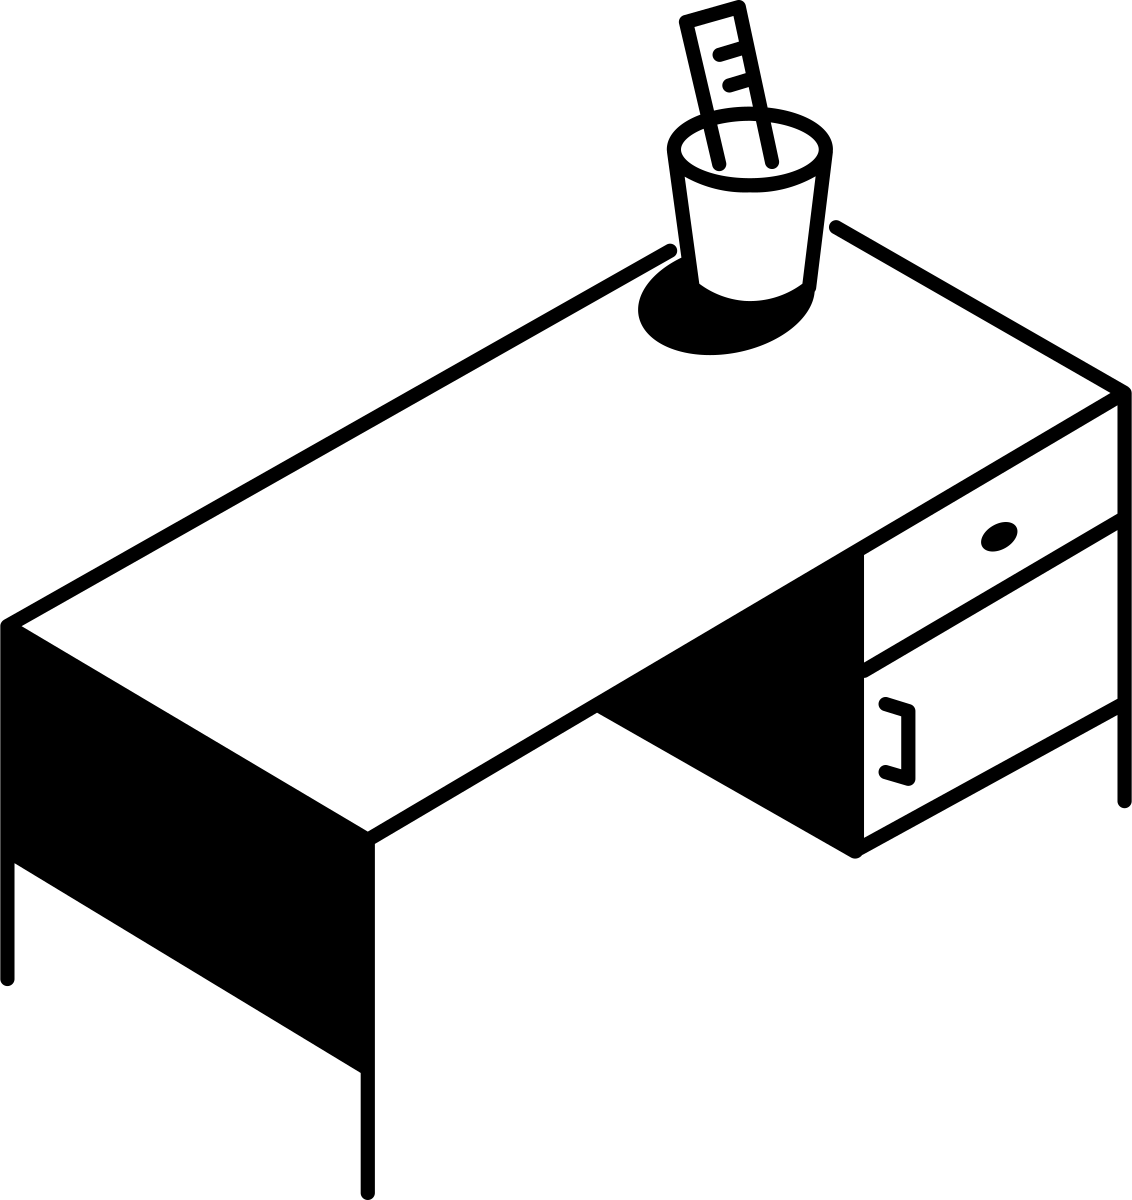
\includegraphics[height=3mm]{clipart/desk} \href{https://thenounproject.com/icon/office-desk-5184572/}{`office desk'}  by \href{https://thenounproject.com/abdul157/}{Abdul Baasith} is licensed under \CCBYthree~ (accessed 6 June 2023)}

\begin{tikzpicture}
\draw (-1,2) coordinate(a);
\draw (-3,1) coordinate(j);
\draw (0,0) node{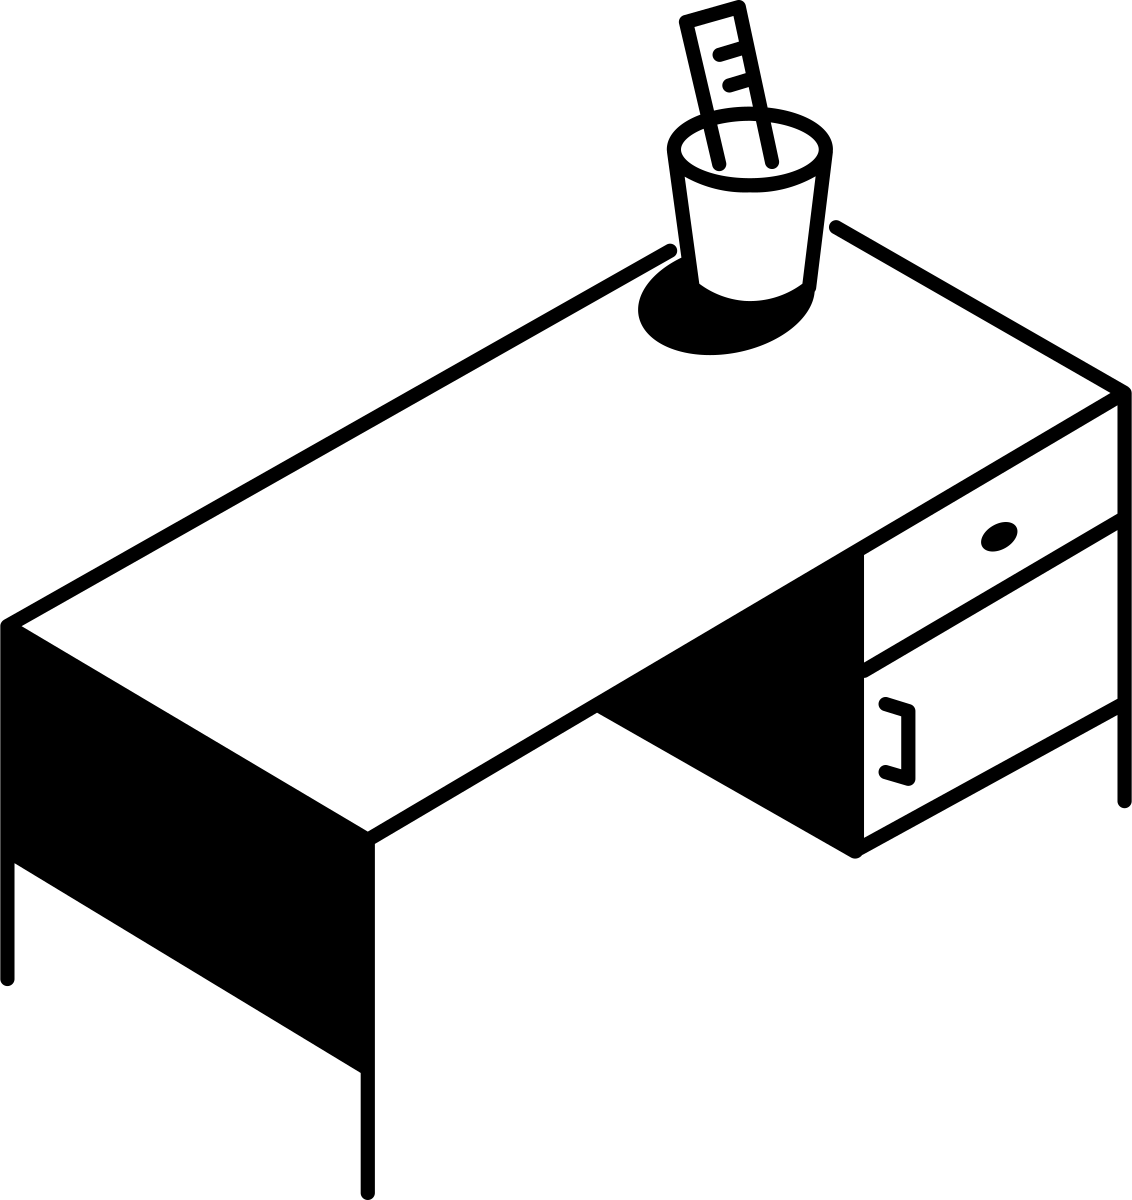
\includegraphics[width=5cm]{clipart/desk}};
%Andrew and his cookies
\onslide<1-2|handout:1>{\draw (a)node{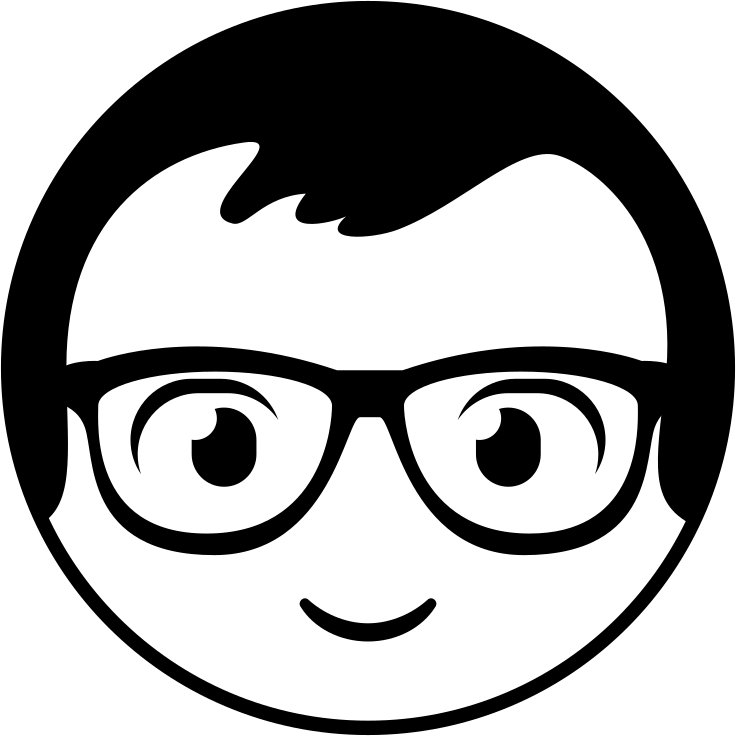
\includegraphics[width=1.5cm]{clipart/andrew}};
\index{ 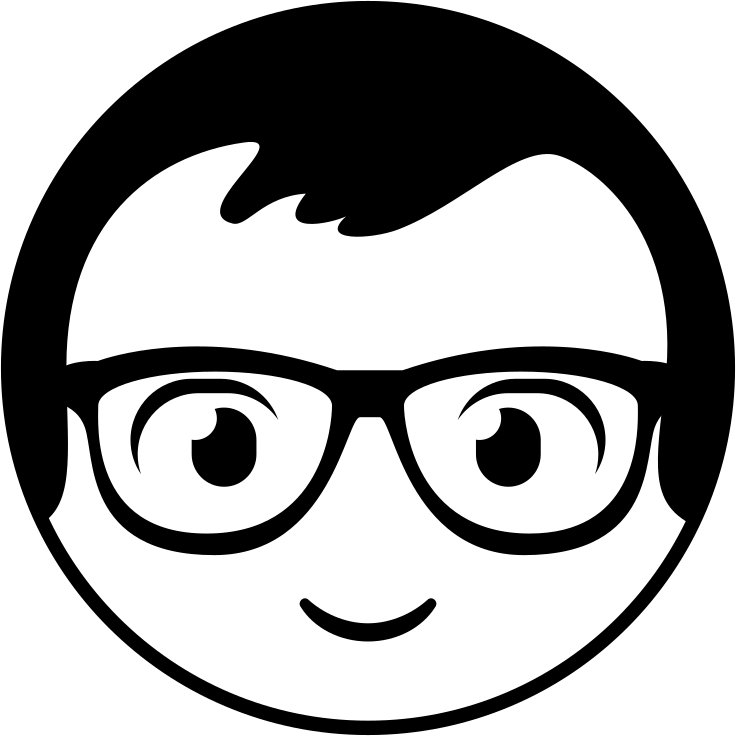
\includegraphics[height=3mm]{clipart/andrew} \href{https://thenounproject.com/icon/boy-4121047/}{`boy'}  by \href{https://thenounproject.com/xinhstudio/}{Xinh Studio} is licensed under \CCBYthree~ (accessed 6 June 2023)}
	}
\draw (.2,.6)node(c1){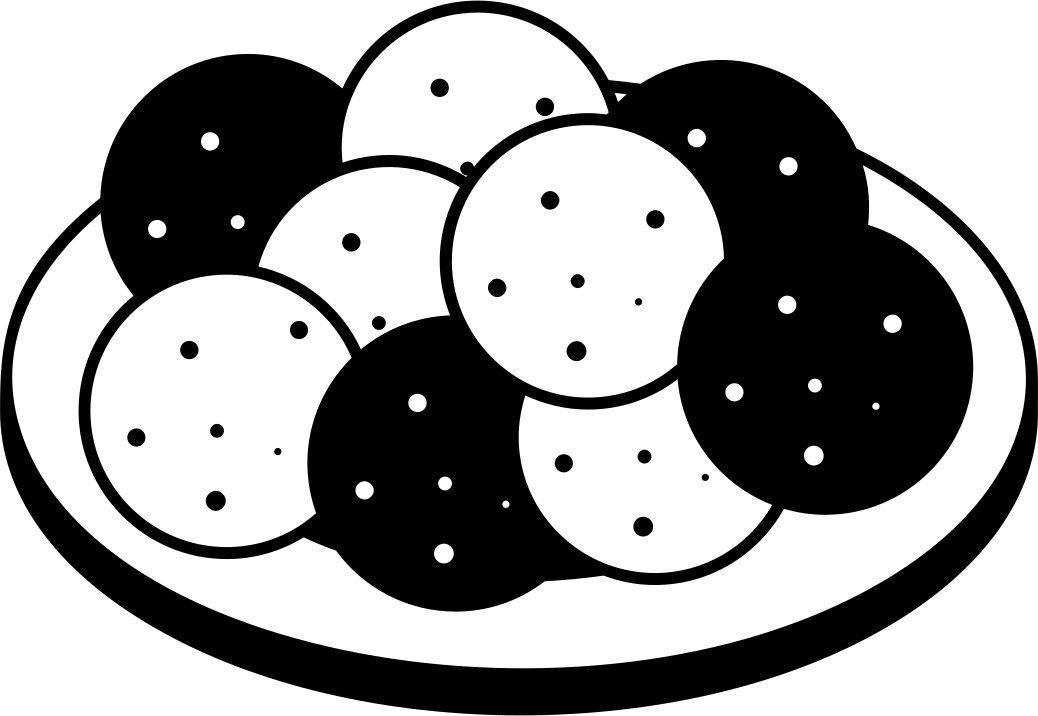
\includegraphics[width=1.25cm]{clipart/cookies1}};
	\index{ 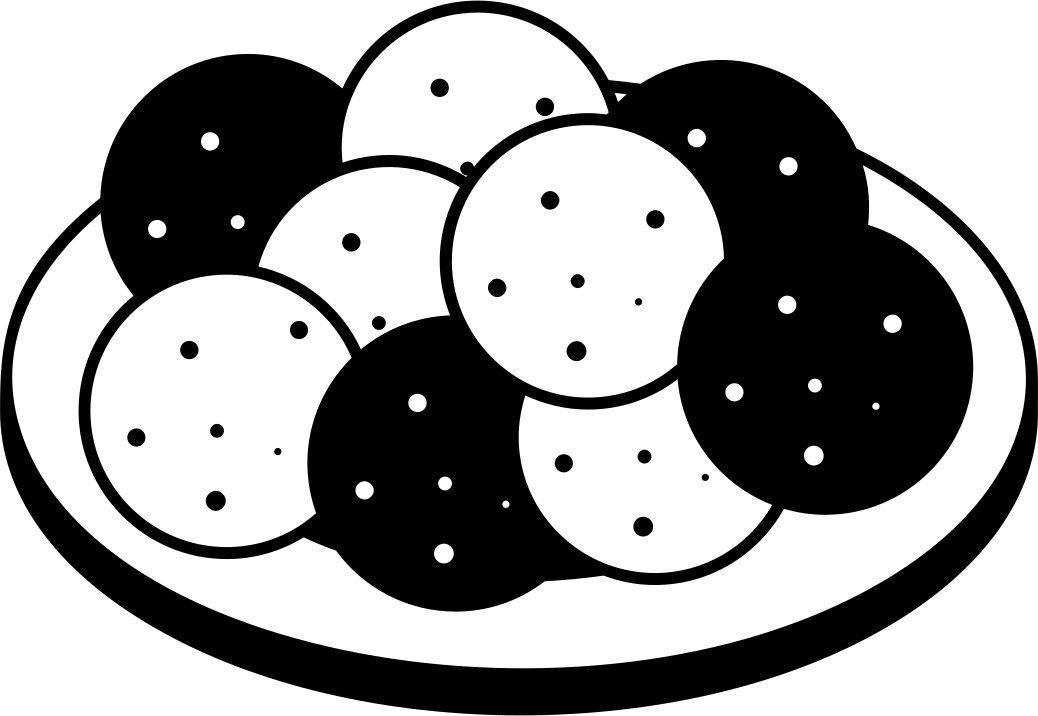
\includegraphics[height=3mm]{clipart/cookies1} \href{https://thenounproject.com/icon/cookies-5762988/}{`cookies'}  by \href{https://thenounproject.com/shmai.com/}{Azam Ishaq} is licensed under \CCBYthree~ (accessed 6 June 2023)}
	\draw (3,2)node[right]{\parbox{4cm}{Andrew brings a plate of cookies to the professor's desk. When he puts them down, there are 10 cookies on the desk.
}};

%Joel and his cookies
\onslide<2|handout:1>{\draw (-3,1)node{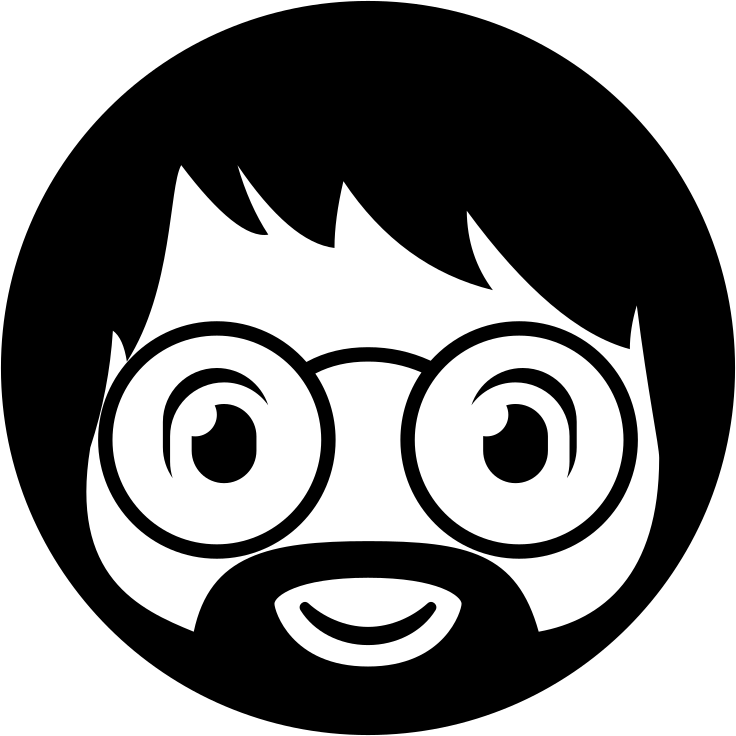
\includegraphics[width=1.5cm]{clipart/joel}};
\index{ 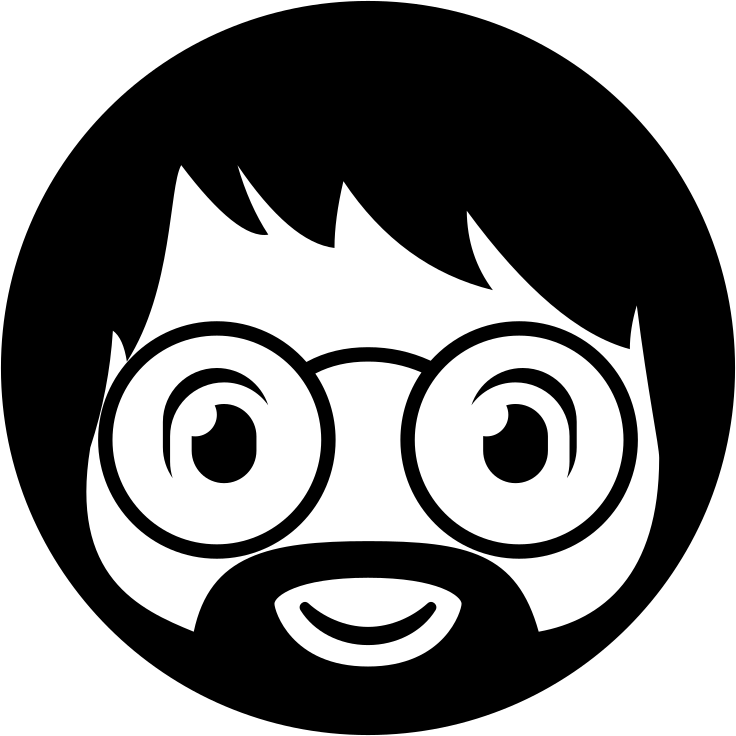
\includegraphics[height=3mm]{clipart/joel} \href{https://thenounproject.com/icon/man-4121059/}{`Man'}  by \href{https://thenounproject.com/xinhstudio/}{Xinh Studio} is licensed under \CCBYthree~ (accessed 6 June 2023)}
	}
\onslide<2-3,5->{
	\draw(-.9,-0.1)node(c2){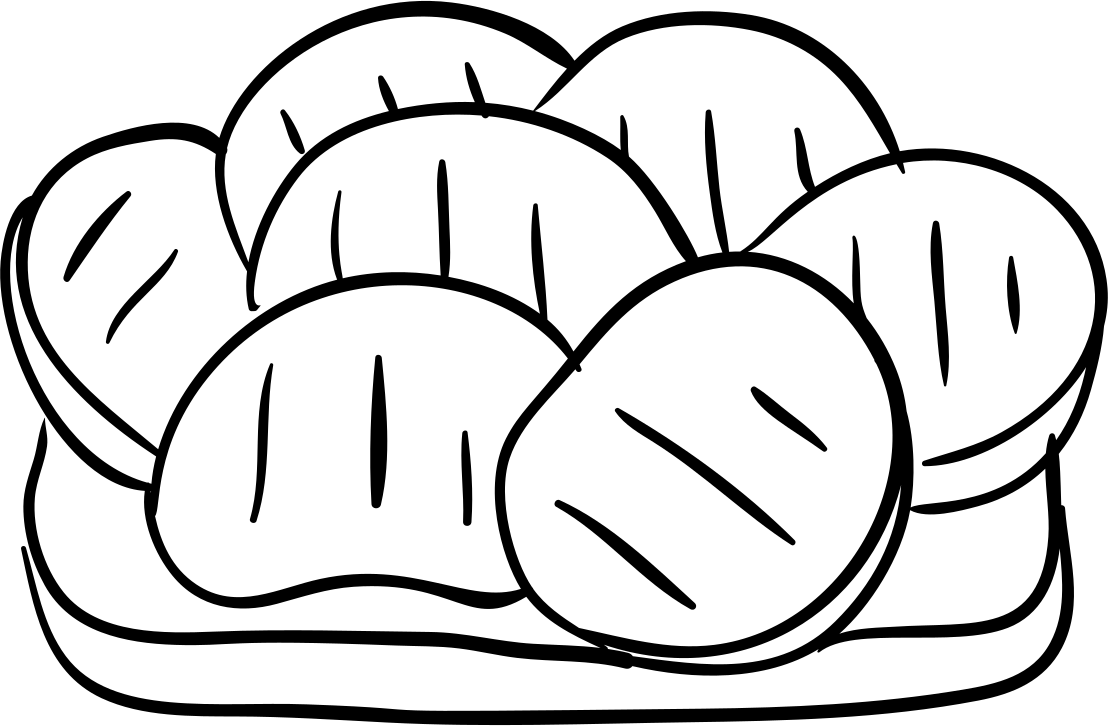
\includegraphics[width=1.25cm]{clipart/cookies2}};
	\index{ 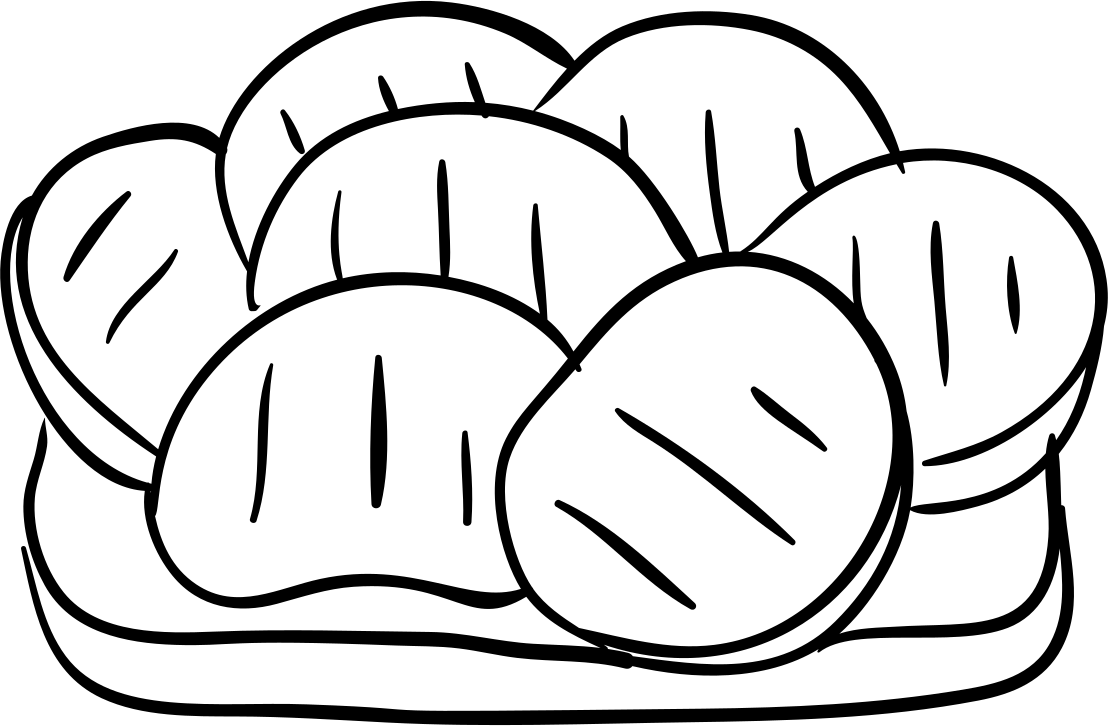
\includegraphics[height=3mm]{clipart/cookies2} \href{https://thenounproject.com/icon/cookies-3151013/}{`cookies'}  by \href{https://thenounproject.com/vectorspoint/}{Vectors Point} is licensed under \CCBYthree~ (accessed 6 June 2023)}}
\onslide<2->{
	\draw (3,-1)node[right]{\parbox{4cm}{Then, Joel brings a plate of cookies. When he puts them down, there are 19 cookies on the desk.\\[1em]
	How many cookies did each person bring?
}};
	}
\onslide<3-|handout:2>{
	\draw(c1) node[fill=white,fill opacity=0.95,shape=ellipse]{\large $a_1$};}
\onslide<3,5-|handout:2>{
	\draw(c2) node[fill=white,shape=ellipse]{\large $a_2$};
	}
\onslide<4-|handout:2>{
	\color{C4}
	\draw[rotate=30,fill,fill opacity=0.2] (c1) circle (8 mm) ;
	\draw(a)node{$S_1=a_1$};
	}
\onslide<5-|handout:2>{
	\color{M5}
	\draw[rotate=30,fill,fill opacity=0.2] (-.2,0.4) ellipse (1.5 and .7) ;
	\draw(j)node[xshift=5mm]{$S_2=a_1+a_2$};
	}
\end{tikzpicture}
\vfill
\sonslide<3->{Andrew brought 10, and Joel brought $19-10=9$.}
\end{frame}
%----------------------------------------------------------------------------------------

%----------------------------------------------------------------------------------------
\begin{frame}[t]{Notation Practice}
\AnswerYes<1>\QuestionBar<1>{2}{2}
\AnswerBar<2>{2}{2}
  Suppose $\ds\sum\limits_{n=1}^\infty a_n$ has partial sums $\ds S_N=\sum\limits_{n=1}^Na_n=\frac{N}{N+1}$.
\begin{itemize}
	\item Find $a_1$.
	\qquad\sonslide<2->{$\ds a_1=\sum_{n=1}^1 a_n=S_{1}=\frac12$}\vfill
	\item Give an explicit expression for $a_n$, when $n>1$.\\
	 \sonslide<2->{\begin{align*}
	 a_n&=\left(\sum_{k=1}^n a_k\right) - \left(\sum_{k=1}^{n-1}a_k\right)=S_{n}-S_{n-1}\\
	 &=\frac{n}{n+1}-\frac{n-1}{n}=\frac{1}{n(n+1)}\end{align*}}\vfill
\end{itemize}

\end{frame}
%----------------------------------------------------------------------------------------
%----------------------------------------------------------------------------------------
\begin{frame}<1-5>{$S_N = \sum\limits_{n=1}^Na_n=\frac{N}{N+1}$}

\StatusBar{1}{5}
\centering

\begin{tikzpicture}
\weights{1.5,1.3,1.1,.9,.7,.5,.3,.1}
{a_1,a_2,a_3,a_4,a_5,a_6,a_7,a_8}
{1/(1+1),2/(2+1),3/(3+1),4/(4+1),5/(5+1),6/(6+1),7/(7+1),8/(8+1)}
\end{tikzpicture}

\end{frame}
%----------------------------------------------------------------------------------------

%----------------------------------------------------------------------------------------
%----------------------------------------------------------------------------------------
%----------------------------------------------------------------------------------------
\begin{frame}[t]
\begin{defn}
The $N^{\rm th}$ partial sum of the series $\sum_{n=1}^\infty a_n$ is the sum of its first $N$ terms
\begin{align*}
S_N=\sum_{n=1}^N a_n.
\end{align*}
The partial sums form a sequence $\big\{S_N\big\}_{N=1}^\infty$.
If this sequence of partial sums converges $S_N \to S$ as
$N\rightarrow\infty$  then we say that the series $\sum_{n=1}^\infty a_n$
converges to $S$ and we write
\begin{equation*}
\sum_{n=1}^\infty a_n=S
\end{equation*}
If the sequence of partial sums diverges, we say that the series diverges.
\end{defn}
\unote{Definition~\eref{text}{def:SRseries}}
\end{frame}
%----------------------------------------------------------------------------------------
\begin{frame}[t]
\begin{block}{Geometric Series}
Let $a$ and $r$ be two fixed real numbers with $a \neq 0$. The series 
\[a+ar+ar^2+ar^3+\cdots\]
is called the \textbf{geometric series} with first term $a$ and ratio $r$.
\end{block}
We call $r$ the \textit{ratio} because it is the quotient of consecutive terms:
\[\frac{ar^{n+1}}{ar^n}=r\]\pause
Another useful way of identifying geometric series is to determine whether all pairs of consecutive terms have the same ratio.

\begin{itemize}
\item  Geometric: $\ds 1+\frac15+\frac{1}{5^2}+\frac{1}{5^3}+\frac{1}{5^4}+\cdots$
\item Geometric: $\ds\sum_{n=0}^\infty \frac{1}{2^n}$
\item Not geometric: $\ds 1 \foreach \d in {2,...,6}{+ \frac1\d}+\cdots$
\end{itemize}
\end{frame}

%----------------------------------------------------------------------------------------
\begin{frame}[t]
\StatusBar{1}{6}
\only<2,4>{\AnswerYes}
Consider the partial sum $S_N$ of a geometric series:
\begin{align*}
S_N&=a+ar+ar^2+ar^3+\cdots +ar^N\\
\onslide<2->{rS_N&=\hspace{6mm}}\onslide<3-|handout:0>{\color{spoilercolor}ar+ar^2+ar^3+\cdots +ar^N+ar^{N+1}}\\
\onslide<4->{rS_N-S_N&=}\onslide<5-|handout:0>{\color{spoilercolor}-a\hspace{19mm}+\hspace{19mm}ar^{N+1}}\\
\onslide<6->{S_N(r-1)&=ar^{N+1}-a\\
\intertext{If $ r \neq 1$, then}
S_N&=\frac{ar^{N+1}-a}{r-1}=a\frac{r^{N+1}-1}{r-1}}
\end{align*}

\end{frame}

%----------------------------------------------------------------------------------------
\begin{frame}[t]
\AnswerYes<1>
\begin{block}{Geometric Series and Partial Sums}
Let $a$ and $r$ be constants with $a \neq 0$, and let $N$ be a natural number.
\begin{itemize}
\item If $r \neq 1$, then $\ds a+ar+ar^2+ar^3+\cdots+ar^N=a\frac{r^{N+1}-1}{r-1}$.
\item If $r = 1$, then $\ds a+ar+ar^2+ar^3+\cdots+ar^N=
\sonslide<2->{(N+1)a.}$
\item If $|r|<1$, then $\ds\sum_{n=0}^\infty ar^n=\sonslide<2->{
\lim_{N \to \infty}a\frac{r^{N+1}-1}{r-1}=a\frac{1}{1-r}}$
\item If $r=1$, then $\ds\sum_{n=0}^\infty ar^n$ \sonslide<2>{ diverges}
\item If $r=-1$, then $\ds\sum_{n=0}^\infty ar^n$ \sonslide<2>{diverges}
\item If $|r|>1$, then $\ds\sum_{n=0}^\infty ar^n$ \sonslide<2>{diverges}
\end{itemize}
\end{block}
\unote{Example~\eref{text}{eg:SRgeom}}
\end{frame}
%----------------------------------------------------------------------------------------
\begin{frame}[t]{$\sum\limits_{n=0}^\infty ar^n$, $r=1$, $a\neq 0$}
\StatusBar{1}{8}

\setpartialstart{0} %%%start from S_0, not S_1, until \resetpartialstart or end of frame
\begin{tikzpicture}
\weights{1,1,1,1,1,1}
{a,a,a,a,a,a}
{$a$,$2a$,$3a$,$4a$,$5a$,$6a$}
\onslide<8-|handout:0>{
\begin{scope}[yshift=2.5cm, yscale=0.8]
\myaxis{N}{0}{5.5}{S_N}{0}{3.1}
\foreach \x[evaluate=\y using int(\x-1)] in {1,...,6}{
	\xcoord{\y}{\y}
	\ifnum \x=1 \ycoord{\x/2}{a}
	\else \ycoord{\x/2}{\x a}
	\fi
	\draw(\y,\x/2)node[vertex]{};
	}
\end{scope}
}
\end{tikzpicture}

\end{frame}

%----------------------------------------------------------------------------------------
\begin{frame}[t]{$\sum\limits_{n=0}^\infty ar^n$, $r=-1$, $a \neq 0$}
\StatusBar{1}{8}
\setpartialstart{0}
\begin{tikzpicture}
\weights{1,-1,1,-1,1,-1}
{a,-a,a,-a,a,-a}
{$a$,$0$,$a$,$0$,$a$,$0$}
\onslide<8-|handout:0>{
\begin{scope}[yshift=3.5cm, yscale=0.8]
\myaxis{N}{0}{5.5}{S_N}{0}{2}
\ycoord{1.75}{a}
\foreach \x in {0,...,5}{\xcoord{\x}{\x}}
\foreach \x[evaluate=\y using \x+1] in {0,2,4}{
	\draw(\x,1.75)node[vertex]{};
	\draw(\y,0)node[vertex]{};}
\end{scope}
}
\end{tikzpicture}
\end{frame}
%----------------------------------------------------------------------------------------
\begin{frame}[t]{$\sum\limits_{n=0}^\infty ar^n$, $r>1$, $a \neq 0$}
\StatusBar{1}{7}
\setpartialstart{0}
\begin{tikzpicture}
\weights{1,1.2,1.4,1.7,2.1}
{a,ar,ar^2,ar^3,ar^4}
{$a$,$a\frac{r^2-1}{r-1}$,$a\frac{r^3-1}{r-1}$,$a\frac{r^4-1}{r-1}$,$a\frac{r^5-1}{r-1}$}
\onslide<7-|handout:0>{
\begin{scope}[yshift=2.5cm,xshift=-5mm]
\myaxis{N}{0}{4.5}{S_N}{0}{2.8}
\foreach \x[evaluate=\y using 2*(1.2^(\x+1)-1)] in {0,...,4}{
	\xcoord{\x}{\x}
	\draw (\x,\y)node[vertex]{};
	}

\end{scope}
}
\end{tikzpicture}
\end{frame}

%----------------------------------------------------------------------------------------
\begin{frame}[t]{$\sum\limits_{n=0}^\infty ar^n$, $r<-1$, $a \neq 0$}
\StatusBar{1}{8}
\setpartialstart{0}
\begin{tikzpicture}
\weights{1,-1.2,1.4,-1.7,2.1,-2.5}
{a,ar,ar^2,ar^3,ar^4,ar^5}
{$a$,$a\frac{r^2-1}{r-1}$,$a\frac{r^3-1}{r-1}$,$a\frac{r^4-1}{r-1}$,$a\frac{r^5-1}{r-1}$,$a\frac{r^6-1}{r-1}$}
\onslide<8-|handout:0>{
\begin{scope}[yshift=4cm,xshift=-5mm,yscale=0.9]
\myaxis{N}{0}{5.5}{S_N}{.5}{1.5}
\foreach \x[evaluate=\y using (-.4*((-1.3)^(\x+1)-1))] in {0,...,5}{
	\xcoord{\x}{\x}
	\draw (\x,\y)node[vertex]{};
	}

\end{scope}
}\end{tikzpicture}
\end{frame}

%----------------------------------------------------------------------------------------
%----------------------------------------------------------------------------------------
\begin{frame}[t]{Geometric Series}
\AnswerYes<1,3>
\nsMoreSpace<1>
\only<-2>{New bitcoins are produced when a particular type of computational problem is solved. Every time 210,000 solutions are found, the number of bitcoins each solution can produce is cut in half.
\snshonly{1-}{1}{1-}{\begin{itemize}
\item Each of the first 210,000 solutions can produce $50$ bitcoins.
\item Each of the next 210,000 solutions can produce $\frac{50}{2}$ bitcoins.
\item  Each of the next 210,000 solutions can produce $\frac{50}{2^2}$ bitcoins.
\item  Each of the next 210,000 solutions can produce $\frac{50}{2^3}$ bitcoins.
\end{itemize}
Assume that this continues forever, and that bitcoins are infinitely divisible.\footnote{Actually the smallest allowed division of a bitcoin is $10^{-8}$.}} How many bitcoins can possibly be produced?}


\sonly<2>{We start by writing the total number of bitcoin produced as a series. Since we want to know an upper bound, we'll assume that infinite solutions can be found and used to make bitcoin.
\[210\,000(50)+210\,000\left(\frac{50}{2}\right)+210\,000\left(\frac{50}{2^2}\right)+\cdots = \sum_{n=0}^\infty (210\,000)\left(\frac{50}{2^n}\right)\]
\MoreSpace
}
\sonly<3->{\begin{align*}
\sum_{n=0}^\infty (210\,000)\left(\frac{50}{2^n}\right)&=\onslide<4->{
\sum_{n=0}^\infty (210\,000\cdot 50)\left(\frac{1}{2}\right)^n\\
&= (210\,000\cdot 50)\frac{1}{1-\frac12}\\
&=(210\,000\cdot 50)(2)\\
&=21\,000\,000
\intertext{So there will never be more than 21,000,000 bitcoins produced this way.}}
\end{align*}
}
\end{frame}
%----------------------------------------------------------------------------------------
%----------------------------------------------------------------------------------------
\begin{frame}[t]
\label<1>{note3.2d}
$\displaystyle\sum_{n=0}^\infty 210\,000\left(\frac{50}{2^n}\right)=21\,000\,000$ 

\begin{center}
\setpartialstart{0}
\begin{tikzpicture}[xscale=1.1]
\weights{5,4,3,2,1}{10\,500\,000,{\text{\small 5\,250\,000}},{\text{\footnotesize2\,625\,000}},{\text{\scriptsize1\,312\,500}},{ \text{\tiny656\,250}}}{10\,500\,000,15\,750\,000,18\,375\,000,19\,687\,500,20\,343\,750}
\end{tikzpicture}
\end{center}
\end{frame}
%----------------------------------------------------------------------------------------
%----------------------------------------------------------------------------------------
\begin{frame}[t]
\begin{block}{Arithmetic of Series}
Let $S$, $T$, and $C$ be real numbers. Let the two series $\sum_{n=1}^\infty a_n$ and $\sum_{n=1}^\infty b_n$ converge to $S$ and $T$ respectively. Then
\[\sum_{n=1}^\infty [a_n+b_n]=S+T\]
\[\sum_{n=1}^\infty [a_n-b_n]=S-T\]
\[\sum_{n=1}^\infty [Ca_n]=CS\]

\end{block}
\unote{Theorem~\eref{text}{thm:SRseriesarith}}
\end{frame}

%----------------------------------------------------------------------------------------
\begin{frame}[t]
\snshonly{1,4,7}{1,3,5}{1-}{\begin{block}{Geometric Series and Partial Sums}
Let $a$ and $r$ be fixed numbers, and let $N$ be a positive integer. Then
\[\sum_{n=0}^N ar^n = \begin{cases}
a\cdot\frac{1-r^{N+1}}{1-r} &\mbox{if }r \neq 1\\
a(N+1) &\mbox{if }r = 1
\end{cases}\]
so
\[\sum_{n=0}^\infty ar^n = \frac{a}{1-r}\mbox{ provided }|r|<1\]
\end{block}}
\only<1|handout:1>{Evaluate $\displaystyle\sum_{n=0}^\infty \left(\frac{2}{3^n}+\frac{4}{5^n}\right)$}
\QuestionBar<1-2|handout:1>{1}{3}
\MoreSpace<1>
\AnswerYes<2>
\snshonly{2-3}{2}{0}{
\AnswerBar{1}{3}
\begin{align*}
\color{black}\sum_{n=0}^\infty\left(\frac{2}{3^n}+\frac{4}{5^n}\right)&=
\onslide<3>{\sum_{n=0}^\infty \frac{2}{3^n}+\sum_{n=0}^\infty \frac{4}{5^n}\\
&=\sum_{n=0}^\infty 2\left(\frac{1}{3}\right)^n+\sum_{n=0}^\infty 4\left(\frac{1}{5}\right)^n\\
&=\frac{2}{1-\frac13}+\frac{4}{1-\frac15}\\
&=\frac{2}{2/3}+\frac{4}{4/5}\\
&=3+5=8
}
\end{align*}
}
\snshonly{4}{3}{2}{Evaluate $\displaystyle\sum_{n=6}^\infty \left(\frac{3^{n-1}}{5^{2n}}\right)$}
\sQuestionBar<4-5>{2}{3}
\sMoreSpace<4>
\nsMoreSpace<3>
\nsQuestionBar<3-4|handout:2>{2}{3}
\AnswerYes<5>
\snshonly{5-6}{4}{0}{
\begin{align*}
\color{black}\sum_{n=6}^\infty \left(\frac{3^{n-1}}{5^{2n}}\right)&=\sonslide<6>{
\sum_{n=6}^\infty \frac13\left(\frac{3^{n}}{5^{2n}}\right)
=\sum_{n=6}^\infty \frac13\left(\frac{3^{n}}{25^{n}}\right)
=\sum_{n=6}^\infty \frac13\left(\frac{3}{25}\right)^n
\intertext{Set $k=n-6$. Then $n=k+6$ and when $n=6$, $k=0$.}
&=\sum_{k=0}^\infty \frac13\left(\frac{3}{25}\right)^{k+6}
=\sum_{k=1}^\infty \frac13\left(\frac{3}{25}\right)^6\left(\frac{3}{25}\right)^k\\
&=\frac13\left(\frac{3}{25}\right)^6\cdot\frac{1}{1-3/25}=
\frac{3^5}{25^6}\cdot\frac{25}{22}=\frac{3^5}{25^5\cdot 22}
}
\end{align*}
\AnswerBar{2}{3}}
\snshonly{7}{5}{3}{Evaluate $\displaystyle\sum_{n=0}^\infty \left(\frac{2^{2n}}{3^{n}}\right)$}
\sQuestionBar<7>{3}{3}
\sMoreSpace<7>
\nsQuestionBar<5-6|handout:3>{3}{3}
\nsMoreSpace<5>
\AnswerYes<8>
\snshonly{8-9}{6}{0}{
\begin{align*}
\color{black}\sum_{n=0}^\infty \left(\frac{2^{2n}}{3^{n}}\right)&=
\sonslide<9>{\sum_{n=0}^\infty \left(\frac{4^{n}}{3^{n}}\right)\\
&=\sum_{n=1}^\infty \left(\frac{4}{3}\right)^n
\intertext{Since $\left| \frac43\right|>1$, the series diverges.}}
\end{align*}
\AnswerBar{3}{3}}

\end{frame}
%----------------------------------------------------------------------------------------%----------------------------------------------------------------------------------------
%----------------------------------------------------------------------------------------
%----------------------------------------------------------------------------------------
\begin{frame}<beamer>
$\displaystyle\sum_{n=0}^\infty \left(\frac{2^{2n}}{3^{n}}\right)$ diverges

\vspace{-1cm}\begin{center}
\setpartialstart{0}
\begin{tikzpicture}
\weights{1,1.33,1.78,2.37,3.16,4.21}{1,\frac{4}{3},\frac{16}{9},\frac{64}{27},\frac{256}{81},\frac{1024}{243}}{1.0000,2.3333,4.1111,6.4815,9.6420,13.856}
\end{tikzpicture}
\end{center}
\end{frame}
%----------------------------------------------------------------------------------------

%----------------------------------------------------------------------------------------

%----------------------------------------------------------------------------------------
%----------------------------------------------------------------------------------------
\begin{frame}[t]{Telescoping Sums}
\sStatusBar{2}{8}
\QuestionBar{1}{2}
\AnswerYes\NoSpace
Evaluate $\displaystyle\sum_{n=1}^{800} \left(\frac{1}{n}-\frac{1}{n+1}\right)$.
\hfill
Evaluate $\displaystyle\sum_{n=1}^{\infty}\left( \frac{1}{n}-\frac{1}{n+1}\right)$.
\sonslide<+(1)->{
\begin{align*}
\begin{array}{ccccc}
a_1:&\frac{1}{1}&-&\textcolor<3->{W3}{\frac{1}{2}}\\[1mm]
a_2:&\textcolor<3->{W3}{\frac{1}{2}}&-&\textcolor<4->{M3}{\frac{1}{3}}\\[1mm]
a_3:&\textcolor<4->{M3}{\frac{1}{3}}&-&\textcolor<5->{M4}{\frac{1}{4}}\\[1mm]
a_4:&\textcolor<5->{M4}{\frac{1}{4}}&-&\textcolor<6->{M5}{\frac{1}{5}}\\[1mm]
\vdots\\
a_{N-1}:&\textcolor<6->{M5}{\frac{1}{N-1}}&-&\textcolor<6->{W1}{\frac{1}{N}}\\[1mm]
a_{N}:&\textcolor<6->{W1}{\frac{1}{N}}&-&\frac{1}{N+1}\\[1mm]
\end{array}\quad
\begin{array}{ccclcc}
S_1=&\onslide<+->{\frac{1}{1}&-&\frac{1}{2}\\[1mm]}
S_2=&\onslide<+->{\frac{1}{1}&-&\frac{1}{3}\\[1mm]}
S_3=&\onslide<+->{\frac{1}{1}&-&\frac{1}{4}\\[1mm]}
S_4=&\onslide<+->{\frac{1}{1}&-&\frac{1}{5}\\[1mm]}
\vdots\\
&\onslide<+->{\vphantom{\frac{1}{1}}\\[1mm]}
S_{N}=&\onslide<+->{\frac{1}{1}&-&\frac{1}{N+1}&=\frac{N}{N+1}\\[1mm]}
\end{array}\end{align*}
}
\sonslide<8->{\[\sum_{n=1}^{800} \left(\frac{1}{n}-\frac{1}{n+1}\right)=S_{800}=\frac{800}{801} \qquad
\sum_{n=1}^{\infty}\left( \frac{1}{n}-\frac{1}{n+1}\right)=\lim\limits_{N \to \infty}S_N=1
\]}

\end{frame}
%----------------------------------------------------------------------------------------
\begin{frame}[t]
\AnswerYes<1>\StatusBar{1}{2}
\QuestionBar{2}{2}
Evaluate $\displaystyle\sum_{n=1}^{1000} \log\left(\frac{n+1}{n}\right).$
\hfill
Evaluate $\displaystyle\sum_{n=1}^{\infty} \log\left(\frac{n+1}{n}\right)$.
\sonslide<+(1)->{
\[\begin{array}{lccclclcc}
a_1&:& \log(2)-\cancel{\log(1)} &\quad & S_1 &=&\log(2)\\
a_2&:& \log(3)-\log(2) &\quad & S_2 &=&\log(3)\\
a_3&:& \log(4)-\log(3) &\quad & S_3 &=&\log(4)\\
\vdots\\
a_{n-1}&:& \log(n)-\log(n-1) \\
a_n&:& \log(n+1)-\log(n) &\quad & S_n &=&\log(n+1)\\
\end{array}\]
So, $\displaystyle\sum_{n=1}^{1000} \log\left(\frac{n+1}{n}\right)=S_{1000}=\log(1001)$ and 
$\displaystyle\sum_{n=1}^{\infty} \log\left(\frac{n+1}{n}\right)=\lim_{n \to \infty }\log(n+1)=\infty$
}

\end{frame}
%----------------------------------------------------------------------------------------
%----------------------------------------------------------------------------------------
\begin{frame}<beamer>
$\displaystyle\sum_{n=1}^\infty \log\left(\frac{n+1}{n}\right)$ diverges

\vspace{-1cm}\begin{center}
\begin{tikzpicture}
\weights{0.69,0.41,0.29,0.22,0.18,0.16,0.13}{\log 2,\log\frac32,\log\frac{4}{3},\log\frac{5}{4},\scriptstyle\log\frac{6}{5},\scriptstyle\log\frac{7}{6},\scriptstyle\log\frac{8}{7}}{0.6931,1.0986,1.3863,1.6094,1.7917,1.9459,2.0794}
\end{tikzpicture}
\end{center}
\end{frame}
%----------------------------------------------------------------------------------------
%----------------------------------------------------------------------------------------
